\documentclass[11pt,letterpaper,titlepage]{article}

\usepackage{geometry}
\geometry{left=2cm,right=2cm,top=2cm,bottom=3cm}

\usepackage{setspace}
\onehalfspacing

\usepackage{multicol}
\setlength{\columnsep}{3em}

\usepackage{booktabs}

\usepackage[table,x11names]{xcolor}

\usepackage{multirow}

\usepackage{pgfgantt}

\usepackage{listings}

\usepackage{xcolor}
\definecolor{vgreen}{RGB}{104,180,104}
\definecolor{vblue}{RGB}{49,49,255}
\definecolor{vorange}{RGB}{255,143,102}

\lstdefinestyle{C-style}
{
    language=C,
    basicstyle=\small\ttfamily,
    keywordstyle=\color{vblue},
    identifierstyle=\color{black},
    commentstyle=\color{vgreen},
    % numbers=left,
    numberstyle=\tiny\color{black},
    numbersep=11pt,
    tabsize=4,
    moredelim=*[s][\colorIndex]{[}{]},
    literate=*{:}{:}1
}

\lstdefinestyle{txt-style}
{
    basicstyle=\small\ttfamily,
    % numbers=left,
    numbersep=11pt,
    tabsize=4,
    moredelim=*[s][\colorIndex]{[}{]},
    literate=*{:}{:}1
}

\usepackage{tikz}
\usetikzlibrary{shapes.geometric, arrows, positioning, fit,calc}
\newcommand*\circled[1]{\tikz[baseline=(char.base)]{
            \node[shape=circle,draw,inner sep=1pt] (char) {#1};}}
            
\usepackage{hyperref}
\hypersetup{
    colorlinks,
    citecolor=black,
    filecolor=black,
    linkcolor=black,
    urlcolor=black
}

\usepackage{pifont}

\usepackage[toc,page]{appendix}

\pagestyle{empty}
\usepackage{tikz}
\usetikzlibrary{shapes.geometric, arrows}

\usetikzlibrary{mindmap,trees}
\usepackage{verbatim}

\usepackage{indentfirst}
\setlength{\parindent}{2em}

\usepackage{listings}

\usepackage{chngcntr}
\counterwithin{section}{part}
\renewcommand\thesection{\arabic{section}}

\usepackage{graphicx}

\usepackage{subcaption}

\usepackage{fancyhdr}

\pagestyle{fancy}
\lhead{}
\rhead{}
\lfoot{ECEN 749 Section 601 Lab 5}
\cfoot{\thepage}
\rfoot{@Lei Wang (Wilson)}
\renewcommand{\headrulewidth}{0pt}
\renewcommand{\headwidth}{\textwidth}
\renewcommand{\footrulewidth}{0.4pt}
\newcommand{\RomanNumeralCaps}[1]
    {\MakeUppercase{\romannumeral #1}}

\makeatletter
\newcommand*\@lbracket{[}
\newcommand*\@rbracket{]}
\newcommand*\@colon{:}
\newcommand*\colorIndex{%
    \edef\@temp{\the\lst@token}%
    \ifx\@temp\@lbracket \color{black}%
    \else\ifx\@temp\@rbracket \color{black}%
    \else\ifx\@temp\@colon \color{black}%
    \else \color{vorange}%
    \fi\fi\fi
}
\makeatother

\usepackage{trace}

\begin{document}

\begin{titlepage}
  \centering
	{\scshape\large Texas A\&M University \par}
	\vspace{1cm}
	{\scshape\Large Department of Electrical and Computer Engineering \par}
	\vspace{4cm}
    \vspace{0.5cm}
	{\huge\bfseries ECEN 749 Microprocessor System Design\par}
	\vspace{4cm}
	{\Large Lab 5 Report (Section 601)\par}
	\vspace{1cm}
	{\Large Student: Lei Wang (Wilson)\par}
	\vspace{1cm}
	{\Large UIN: 829009485\par}
	\vspace{1cm}
	{\Large Instructor: Dr. Paul V. Gratz\par}
	\vspace{4cm}
	\vfill

  % Bottom of the page
	{\large Submitted: February 25th, 2020 \par}

\end{titlepage}

\newpage

\tableofcontents{}

\newpage

\part{Introduction}

Lab 5 teaches how to write, compile, load and unload Linux kernels on the ZYBO Z7-10 board. The lab is an extension of the previous lab that teaches how to boot Linux from a micro-SD card. Lab 5 consists of building and using two Linux kernels: the hello-world kernel and the multiplier kernel that uses the multiplier IP created back a few labs before.

\part{Procedure}

\begin{enumerate}
    
    \item Preparation and test:
    
    \begin{enumerate}
        
        \item Create a new directory for this lab. Copy all the files from lab4. The sub-directories containing Linux and u-boot may be too large and take a long time to transfer. Leave those sub-directories out. We can bypass such issue by editing the relative path in the makefile.
        
        \item Copy the four files created in lab4 into the micro-SD card.
        
        \item Put the micro-SD card into the ZYBO Z7-10 board and power up the board. A successful boot should be indicated by the green LDE indicating ``programming done''.
        
        \item Run:
        
        \verb|source /opt/coe/Xilinx/Vivado/2015.2/settings64.sh|
        
        \verb|picocom -b 115200 -r -l /dev/ttyUSB1|
        
        \item Press the PS reset button and wait for console output in Picocom.
        
        \item Run:
        
        \verb|mount /dev/mmcb1k0p1 /mnt/|
        
        to mount the micro-SD card into the Linux file system.
        
        \item Run:
        
        \verb|cd /mnt/|
        
        \verb|ls -al|
        
        to check whether the micro-SD card has been properly mounted.
        
        \item Run:
        
        \verb|cd /|
        
        \verb|umount /mnt|
        
        to unmount the micro-SD card.
        
    \end{enumerate}
    
    \newpage
    
    \item The hello kernel:
    
    \begin{enumerate}
        
        \item Pop the micro-SD card after unmounting it and insert into the workstation in the lab. Keep the ZYBO Z7-10 board powered.
        
        \item Create a sub-directory in the lab5 directory named \textbf{module}.
        
        \item Place the \textbf{hello.c} file downloaded from the course website into the created sub-directory.
        
        \item In the same sub-directory, create a makefile with the content in appendix \ref{appendix:makefile_hello}
        
        \item Run:
        
        \verb|source /opt/coe/Xilinx/Vivado/2015.2/settings64.sh|
        
        \verb|make ARCH=arm CROSS COMPILE=arm-xilinx-linux-gnueabi-|
        
        to cross-compile the hello kernel.
        
        \item Copy the \textbf{hello.ko} file to the micro-SD card.
        
        \item Eject the micro-SD card. Insert into the ZYBO Z7-10 board and mount it to the file system.
        
        \item Run
        
        \verb|cd /mnt|
        
        to move to the directory that contains the compiled module.
        
        \item Run the following command to test for loading and unloading kernel modules:
        
        \begin{table}[ht]
        \centering
        \begin{tabular}{@{}lll@{}}
        \toprule
        Command & Comment                              & Example \\ \midrule
        \verb|insmod <module.ko>|        & Install the module                   & \verb|insmod hello.ko|        \\ \midrule
        \verb|lsmod|        & List the installed modules           & \verb|lsmod|        \\ \midrule
        \texttt{dmesg |tail}        & Show the Linux kernel buffer message &    \texttt{dmesg |tail}    \\ \midrule
        \verb|rmmod <module>|        & Remove the module from the kernel    &   \verb|rmmod hello|      \\ \bottomrule
        \end{tabular}
        \caption{Some Linux commands related to kernel modules.}
        \end{table}
        
        to see the output when installing the hello module.
        
        \item Run:
        
        \verb|mkdir -p /lib/modules/`uname -r`|
        
        \verb|rmmod hello|
        
        to remove the \textbf{hello} module from Linux kernel. If the first line is not run, the user is unable to remove an installed module.
        
    \end{enumerate}
    
    \item The multiply kernel:
    
    \begin{enumerate}
        
        \item Create a new folder called \textbf{lab5b} with \textbf{modules} directory copied from the \textbf{lab5} folder.
        
        \item Create a \textbf{multiply.c} file with content listed in appendix \ref{appendix:sourcecode_multiply}.
        
        \item Change the content in \textbf{Makefile} to the one in appendix \ref{appendix:makefile_multiply}.
        
        \item Repeat steps for loading, check kernel message and unloading module.
        
    \end{enumerate}
    
\end{enumerate}

\newpage

\part{Results}

\begin{figure}[ht]
    \centering
    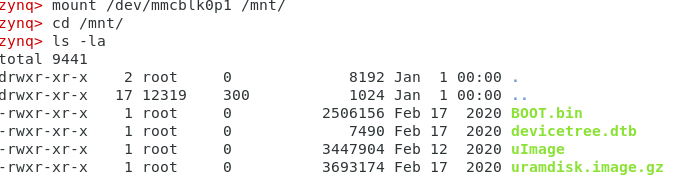
\includegraphics[width=0.8\textwidth]{1.Load_Micro_SD_Card.png}
    \caption{Mount micro-SD card.}
\end{figure}

\begin{figure}[ht]
    \centering
    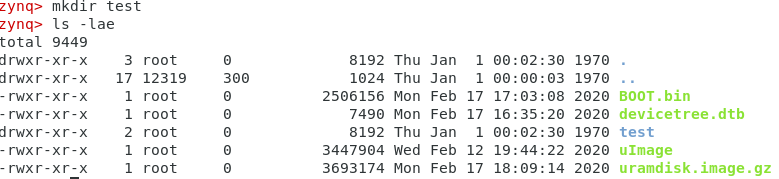
\includegraphics[width=0.8\textwidth]{2.Make_New_Dir.png}
    \caption{Make a new directory \textbf{test} after the micro-SD card is mounted.}
\end{figure}

Note the time associated with directory \textbf{test} is the 1st of January, 1970. This time instant is the start time for Unix operating systems. Linux has the same start time, or time zero, as the Unix does.

\begin{figure}[ht]
    \centering
    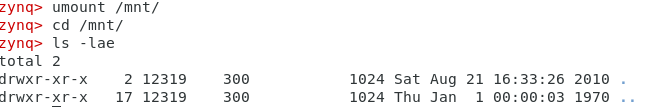
\includegraphics[width=0.8\textwidth]{3.Unmount_Micro_SD_Card.png}
    \caption{Unmount micro-SD card.}
\end{figure}

After the micro-SD card is unmounted, \verb|cd /mnt/| then \verb|ls -lae| or simply \verb|ls /mnt/| shows nothing related to the content in the micro-SD card saw early.

\begin{figure}[h!]
    \centering
    
\includegraphics[width=0.8\textwidth]{4.Check_New_Dir.png}
    \caption{Chech micro-SD card on CentOS workstation.}
\end{figure}

Checking on the CentOS workstation: the newly created \textbf{test} folder is found in the micro-SD card.

\newpage

\begin{figure}[ht]
    \centering
    \begin{subfigure}[b]{0.49\textwidth}
    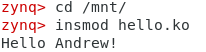
\includegraphics[width=0.49\textwidth]{5.Load_Hello_Module.png}
    \caption{Load the compiled \textbf{hello} module.}
    \end{subfigure}
    \begin{subfigure}[b]{0.49\textwidth}
    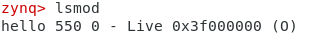
\includegraphics[width=0.7\textwidth]{7.lsmod.png}
    \caption{List the installed modules.}
    \end{subfigure}
    \begin{subfigure}[b]{\textwidth}
    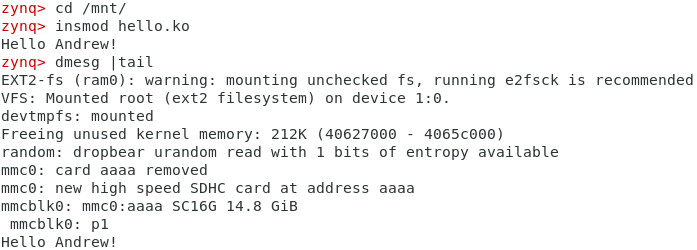
\includegraphics[width=0.8\textwidth]{6.Show_Kernel_Message.png}
    \caption{Show the kernel message after loading the \textbf{hello} module.}
    \end{subfigure}
    \caption{Load, show kernel message and list modules.}
\end{figure}

\begin{figure}[ht]
    \centering
    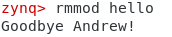
\includegraphics[width=0.2\textwidth]{8.rmmod.png}
    \caption{Remove the \textbf{hello} module.}
\end{figure}

\begin{figure}[ht]
    \centering
    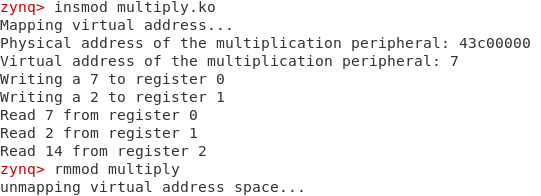
\includegraphics[width=0.8\textwidth]{9.Multiplier.png}
    \caption{Picocom output for loading the \textbf{multiply} kernel.}
\end{figure}

\newpage

\part{Conclusion}

Lab 5 teaches students how to code, compile and run kernel modules in an embedded Linux environment. Operations such as memory mapping is needed since the kernel memory space is separated from the program memory space, or from the hardware memory space, since in Linux, hardware is represented as files and hence has memory address associated with.

A kernel module consists of at least two functions: one called at installing and the other called at removing time. Those functions need to deal with memory mapping or unmapping for releasing resources. 

Compared with previous labs, this lab adds Linux as the interface between the C program and the hardware. Without Linux, it is possible to execute a C program directly, i.e. in a bare-metal way. With Linux, program has to interface with hardware through kernel modules such as device drivers. Pros and cons: an operating system is more flexible and brings more convenient features such as the file system but can cost extra power and hardware resource to run, may impair performance on the execution of the program.

During the lab session, one TA kindly pointed out the significance of the time associated with the newly created folder being the 1st of January, 1970. It is used as the reference for operations that capture time instance. This number can be configured. However, after powering cycle the board, the configuration may be lost. If there is a battery to power the clock on the board, the clock configuration can remain and increment with real-world time lapse.

\textbf{Q: Change thecurrent directory to `/mnt' using `cd' and examine the contents of the directory using `ls'. What do you see?}

A: The setting of the question is after the micro-SD card being unmounted. The output is nothing as the files in the micro-SD card no longer associates with the path \verb|/mnt|.

\textbf{Q: If prior to step 2.f, we accidentally reset the ZYBO Z7-10 board, what additional steps would be
needed in step 2.g?}

A: Steps invloving mounting the micro-SD card to \verb|/mnt| need to be repeated.

\textbf{Q: What is the mount point for the SD card on the CentOS machine?}

A: The micro-SD card is mounted at \verb|/dev/mmcb1k0p1|.

\textbf{Q: If we changed the name of our hello.c file, what would we have to change in the Makefile? Likewise, if in our Makefile, we specified the kernel directory from lab 4 rather than lab 5, what
might be the consequences?}

A: The output object name ending with \textbf{.o} needs to be modified to the new name of the \textbf{.c} file. If the kernel directory is set to lab4, the compilation of the kernel module should carry on as it always does. I am using relative directories to point to the kernel directory from lab 4 on purpose because it takes forever to copy the kernel files from one directory to another and hence I simply skip copying files by instead editing the path pointing to the kernel directory. Possible consequences caused by poorly written Makefile may compile the kernel module and place the object file in other folders instead of the current working directory.

\newpage

\begin{appendices}

\end{appendices}

\section{Makefile for hello.c}
\label{appendix:makefile_hello}
\lstinputlisting[style={txt-style}]{Makefile_hello}

\section{Makefile for multiply.c}
\label{appendix:makefile_multiply}
\lstinputlisting[style={txt-style}]{Makefile_multiply}

\section{multiply.c}
\label{appendix:sourcecode_multiply}
\lstinputlisting[style={txt-style}]{multiply.c}

\end{document}
